\documentclass{article}

\usepackage{graphicx}
\usepackage{pdflscape}
\usepackage[pass]{geometry}
\usepackage{pdfpages}
\usepackage{textgreek}
\usepackage{hyperref}
\setlength{\parskip}{1em}

\begin{document}

	\title{EMISY project report:\\Thermal-paper-based optical storage medium
	reading device}
	\author{Michał Szopiński\\\\
	https://github.com/Lachcim/szopinski-emisy}
	\date{April 2, 2021}
	\maketitle
	
	\setcounter{section}{-1}
	\section{Abstract}
	
	The goal of this project was to design a device capable of reading binary
	data from a tape of 80-millimeter thermal paper on which information is
	encoded as a series of black and white squares. The device was to
	communicate with the host computer over the Universal Serial Bus, which
	would enable the data to be collected and recorded by a dedicated computer
	program.
	
	Described in this document are the engineering challenges faced during the
	construction of the machine as well as detailed descriptions of their
	solutions. The project was successfully completed using real hardware.
	
	\newpage
	\newgeometry{left=2.5cm,right=2.5cm}
	
	\hspace{0cm}
	\vfill
	\begin{figure}[h]		
		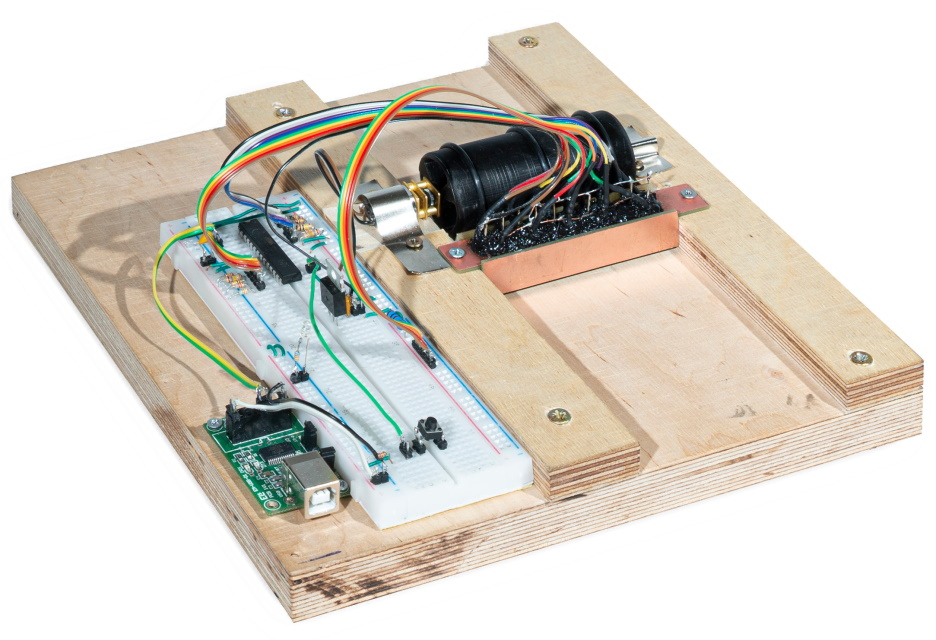
\includegraphics[width=\linewidth]{img/device}
		\caption{A photo of the device.}
	\end{figure}
	\vfill
	\hspace{0cm}
	
	\restoregeometry
	
	\newpage
	\renewcommand{\baselinestretch}{0}\normalsize
	\tableofcontents
	\renewcommand{\baselinestretch}{1}\normalsize
	
	\newpage
	\section{Introduction}
	
	Among the first storage media ever used in computing were punched cards and
	punched tape. Although simple in concept, these media are difficult to read
	quickly and accurately using analog circuitry alone. Combining the
	straightforwardness of the past with the robustness of the present, a
	simple microcontroller system may be devised to ensure that they are
	processed in a swift and reliable manner.
	
	To simplify and accelerate the production of sample media to be used with
	the device, thermal paper was chosen in place of the punched tape. Owing to
	the ubiquity and simplicity of generic point-of-sale linear thermal
	printers, any modern computer may be used to produce data tapes without the
	need for any additional drivers.
	
	Both reading and writing of the data tapes is achieved using a simple
	command line interface utility named \texttt{thermfile}, which comes
	bundled with the source code for this project. The implementation of said
	program is outside the scope of this document.
	
	\subsection{Description of the data format}
	\label{sec:format}
	
	Below is an illustration showing an example data tape with an explanation
	of its characteristic features. As the device pulls the tape through the
	read head, the symbols are scanned from top to bottom.
	
	As seen on figure~\ref{fig:horizontal}, the tape is split into 10
	machine-readable data tracks and an extra human-readable text track. The
	leftmost 8 tracks encode the 8 bits of a byte, with the least significant
	bit towards the right. The text track provides a handy reference as to what
	data is represented by each symbol.
	
	Because the machine has no control over the absolute position of the tape
	and can only approximately control its speed, a synchronization signal must
	be introduced to ensure that the symbols are read correctly. A pattern of
	alternating ones and zeros is printed on the sync track, marking the start
	and end of a symbol.
	
	Finally, the invert track is used to signify that the data bits of a symbol
	are logically inverted, i.e., ones are represented by zeros and vice-versa.
	This is due to a technical limitation of thermal printers whereby an
	excessive burn area causes a voltage drop in the printer's power rail,
	deteriorating the printout quality. The invert track ensures that at most
	50\% of horizontal space is only ever utilized.
	
	\begin{landscape}
		\begin{figure}[h]
			\minipage{0.5\textwidth}
				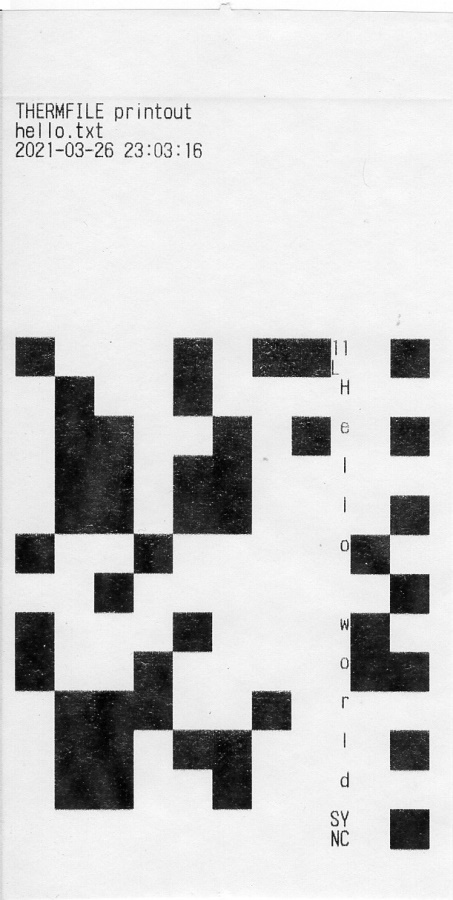
\includegraphics[width=\linewidth]{img/helloworld}
				\caption{Sample data tape}
			\endminipage\hfill
			\minipage{0.5\textwidth}
				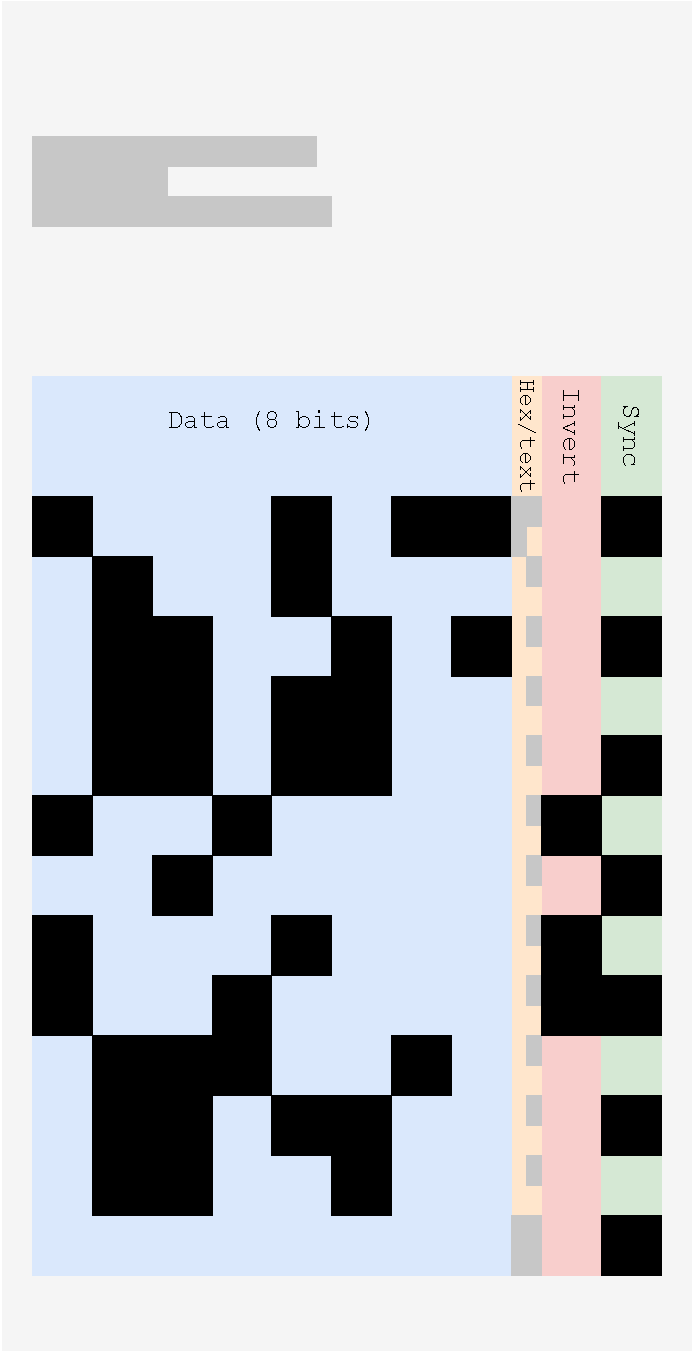
\includegraphics[width=\linewidth]{img/horizontal}
				\caption{Horizontal layout}
				\label{fig:horizontal}
			\endminipage\hfill
			\minipage{0.5\textwidth}
				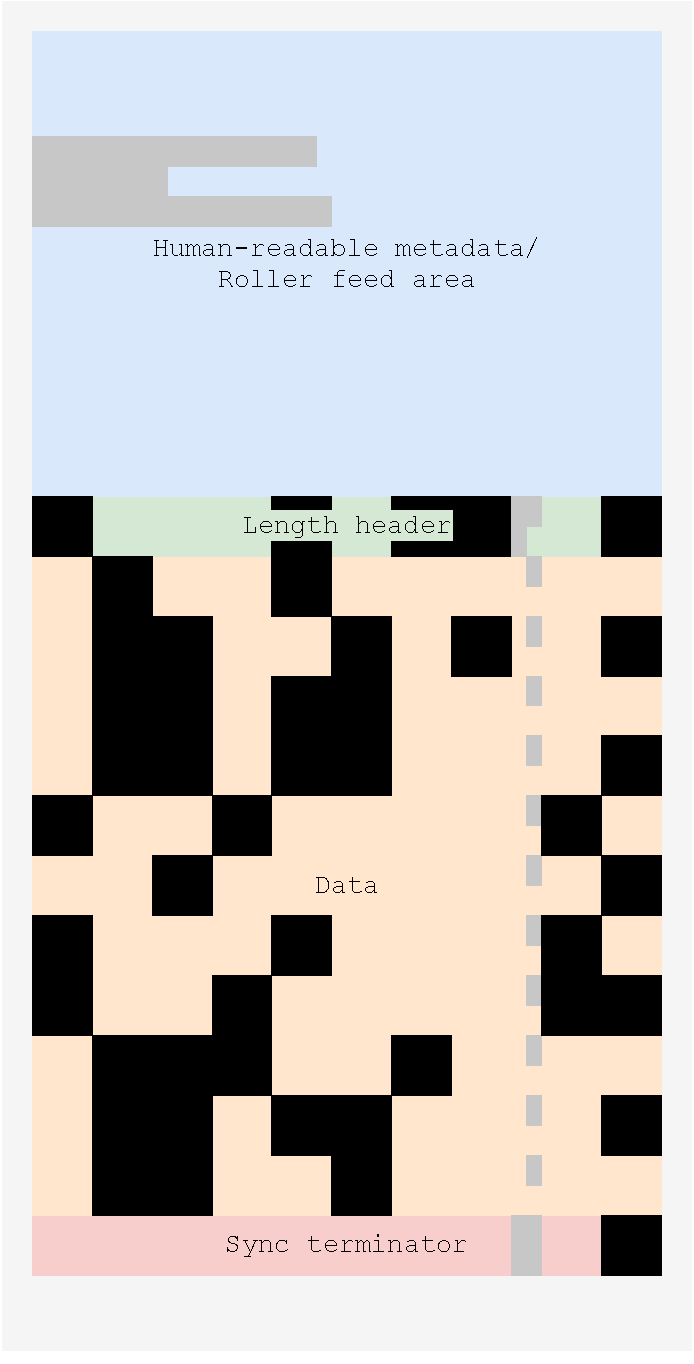
\includegraphics[width=\linewidth]{img/vertical}
				\caption{Vertical layout}
				\label{fig:vertical}
			\endminipage
		\end{figure}
	\end{landscape}
	
	Figure~\ref{fig:vertical} shows the vertical layout of symbols on the tape.
	Each printout begins with a large blank area on which human-readable
	metadata is printed for convenience. This area allows the user to push the
	tape through the read head chamber, past which it can be taken up by the
	roller. It also participates in the two-step read initialization process
	discussed in section~\ref{sec:init}.
	
	As a simple error detection measure, the device is informed about the
	length of the incoming data in advance. This information is carried by the
	length header, present at the start of the data track. Each line of the
	header carries 7 bits of the length value, in little endian order. The
	most significant bit marks the end of the length header.
	
	Past the header, binary data begins. The start and end positions of a
	symbol are determined by detecting a change in the synchronization signal.
	If there is an odd number of symbols on the tape, the final sync signal is
	white and therefore indistinguishable from the white margin of the tape.
	For this reason, a sync terminator is introduced to mark the end of
	odd-numbered final symbols.
	
	\subsection{Communication protocol}
	
	Having no hardware resources required for independent operation, the device
	is granted very little autonomy in terms of its work cycle. The only
	physical control present on its body is the emergency stop button --
	otherwise, session initialization and data collection are both governed by
	the host computer.
	
	A simple communication protocol is used to exchange data and status
	messages with the \texttt{thermfile} utility running on the computer. Each
	packet begins with a single byte identifying the type of the message
	followed by a fixed-size payload. The messages enter and leave the
	microcontroller through UART. USB communication is handled by specialized
	hardware and software.
	
	\newpage
	\subsubsection{Table of messages}
	\label{sec:messages}
	
	\begin{center}
	\begin{tabular}{ |c|c|p{7cm}|c| }
		\hline
			Code & Direction & Meaning & Payload \\
		\hline
			\texttt{S} &
			To device &
			\textbf{Start read}\newline
			Enables power to the read head and starts the roller motor. Begins
			the read session.
			& 0 \\
		\hline
			\texttt{C} &
			To host &
			\textbf{Start read confirm}\newline
			Confirms the start read instruction.
			& 0 \\
		\hline
			\texttt{L} &
			To host &
			\textbf{Incoming data length}\newline
			Announces the length of the incoming data. The payload is a 64-bit
			little-endian value describing the length.
			& 8 \\
		\hline
			\texttt{D} &
			To host &
			\textbf{Incoming data}\newline
			Marks a single byte of the incoming data.
			& 1 \\
		\hline
			\texttt{F} &
			To host &
			\textbf{Read finished}\newline
			Sent once the read session is finished and a new session may be
			initialized.
			& 0 \\
		\hline
			\texttt{E} &
			To host &
			\textbf{Error}\newline
			Signals an error which caused the read session to abort. See the
			table of error codes below.
			& 1 \\
		\hline
			\texttt{X} &
			To device &
			\textbf{Emergency stop}\newline
			Triggers an emergency stop error and halts the read session. The
			device responds with an error code.
			& 0 \\
		\hline
	\end{tabular}
	\end{center}
	
	\subsubsection{Table of error codes}
	
	\begin{center}
	\begin{tabular}{ |c|p{9cm}| }
		\hline
			Error code & Meaning \\
		\hline
			\texttt{I} &
			\textbf{Initialization timeout}\newline
			The first symbol failed to appear within the set timeframe. \\
		\hline
			\texttt{R} &
			\textbf{Read timeout}\newline
			The next symbol failed to appear within the set timeframe. \\
		\hline
			\texttt{E} &
			\textbf{Emergency stop}\newline
			An emergency stop was triggered either by the stop button or
			remotely. \\
		\hline
			\texttt{B} &
			\textbf{Serial buffer busy}\newline
			An attempt to send data was made before the serial buffer had been
			cleared. This error is indicative of a too high scan rate and does
			not occur under ordinary working conditions.\\
		\hline
		\end{tabular}
	\end{center}
	
	\section{Hardware implementation}
	
	\subsection{Choice of microcontroller}
	
	At the heart of the system lies the ATmega328P, a microcontroller from the
	8-bit AVR family of MCUs formerly manufactured by Atmel. This chip was
	chosen based on the following considerations:
	\begin{enumerate}
		\item The vast ubiquity and popularity of the chip which ensure the
		availability of up-to-date documentation and other text resources.
		\item The availability of a well-established, modern and open-source
		programming environment in the form of \texttt{avr-gcc},
		\texttt{avrdude} and USBasp.
		\item The presence of an in-system programming feature which makes
		rapid prototyping possible.
		\item A dual in-line package variant which enables the chip to be
		placed on a breadboard.
		\item 23 general-purpose I/O pins, 18 of which are utilized by the
		device.
		\item 2 kilobytes of RAM and 32 kilobytes of program memory provided a
		wide margin of error before the exact requirements were known.
	\end{enumerate}
	
	A chip from the Intel 8051 family was also briefly considered, but it was
	ultimately rejected due to a lack of a modern open-source environment.
	
	It is now known that a lower-spec ATmega chip such as the ATmega48A is also
	suitable. The ATtiny2313A is a valid candidate as well.
	
	\subsection{General overview of the system}
	
	As described in section~\ref{sec:format}, the device scans the paper tape
	from top to bottom and decodes the symbols printed therein. This involves
	putting the tape into linear motion and periodically probing the light
	intensity of each of the 10 tracks until all the symbols have been scanned.
	
	\begin{figure}[h]
		\begin{center}
			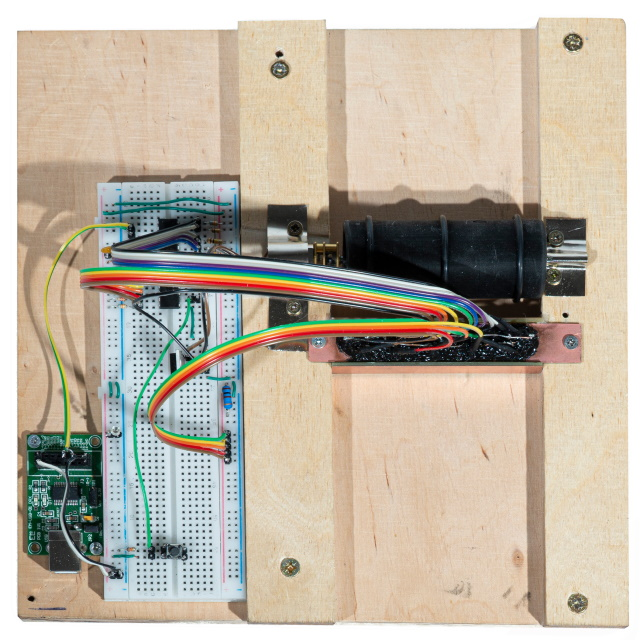
\includegraphics[width=0.75\linewidth]{img/topview}
			\caption{The device as seen from above.}
			\label{fig:topview}
		\end{center}
	\end{figure}
	
	Figure~\ref{fig:topview} shows the top view of the device. Linear motion is
	achieved by pulling the tape through an 80-millimeter-wide trough, which
	ensures that the tracks do not become misaligned with the read head. A DC
	motor coupled with a rubber-coated roller pulls the tape as it passes under
	the head.
	
	\newpage
	
	Suspended above the tape is the read head itself. It consists of 10
	phototransistors aligned with each of the tracks, as well as 5
	light-emitting diodes to provide controllable light conditions. The
	transistors are protected from overexposure by a layer of silicone coating
	from above and a heat shrink tube wrapped around the lens.
	
	\begin{figure}[h]
		\begin{center}
			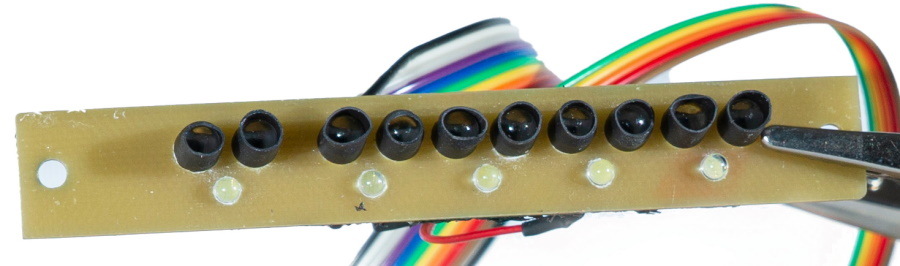
\includegraphics[width=0.75\linewidth]{img/readhead}
			\caption{The front face of the read head.}
			\label{fig:readhead}
		\end{center}
	\end{figure}
	
	To further protect the sensors from interference from outside light
	sources, the read head is enclosed within a dark chamber. The tape enters
	the chamber through a slit where the walls meet the trough. The slit also
	keeps the paper flush with the bottom of the trough.
	
	USB communication, being outside the scope of the project itself, is
	outsourced to an FT232 chip which emulates ordinary RS-232 communication
	over the Universal Serial Bus. The device appears as a serial port
	connection to the host computer. Because the FT232 chip does not come in a
	dual in-line package, a separate PCB is mounted alongside the breadboard.
	
	Being a peripheral device meant to be paired with a desktop computer, the
	reader has no external power source other than the USB port. The FT232 chip
	is configured to permit a maximum current of 500 mA, which is sufficient to
	power the motor even when it is stalled. The current consumed by the LEDs
	is very low (around 20 mA).
	
	The remaining two user-facing features of the device are the emergency stop
	button and the power LED. The button may be pressed to immediately halt a
	read session. The power LED is placed between the power rail and the ground
	rail to indicate that the device is powered on.
	
	\subsection{Detailed discussion}
	
	Below is a schematic fully describing the circuit comprised by the device.
	
	\subsubsection{Microcontroller setup}
	
	The microcontroller is connected to the power rail through a 100 nF
	decoupling capacitor. The power is supplied from the FT232 breakout board,
	which itself also contains circuitry needed to eliminate noise from the
	USB cable. The $AV_{cc}$ pin, while connected, does not require a
	decoupling capacitor because the analog to digital converter is not
	utilized.
	
	To simplify the circuit, no external crystal oscillator is connected to the
	XTAL pins. With the clock prescaler set to 1, the internal RC oscillator
	drives the CPU at 8 MHz, which gives it sufficient computing power to
	perform its tasks in a timely manner.
	
	The $\overline{RESET}$ pin is pulled high through a 10 k\textOmega {}
	pull-up resistor, preventing the controller from resetting. It may be
	driven low by an ISP programmer to force the microcontroller into
	programming mode. The MISO, MOSI and SCK pins are reserved for the ISP
	connector.
	
	Pins RXD and TXD (PD0 and PD1) are used for UART communication with the
	FT232 module. 12 of the remaining 17 pins are used for interacting with the
	environment, 11 of which are configured as inputs.
	
	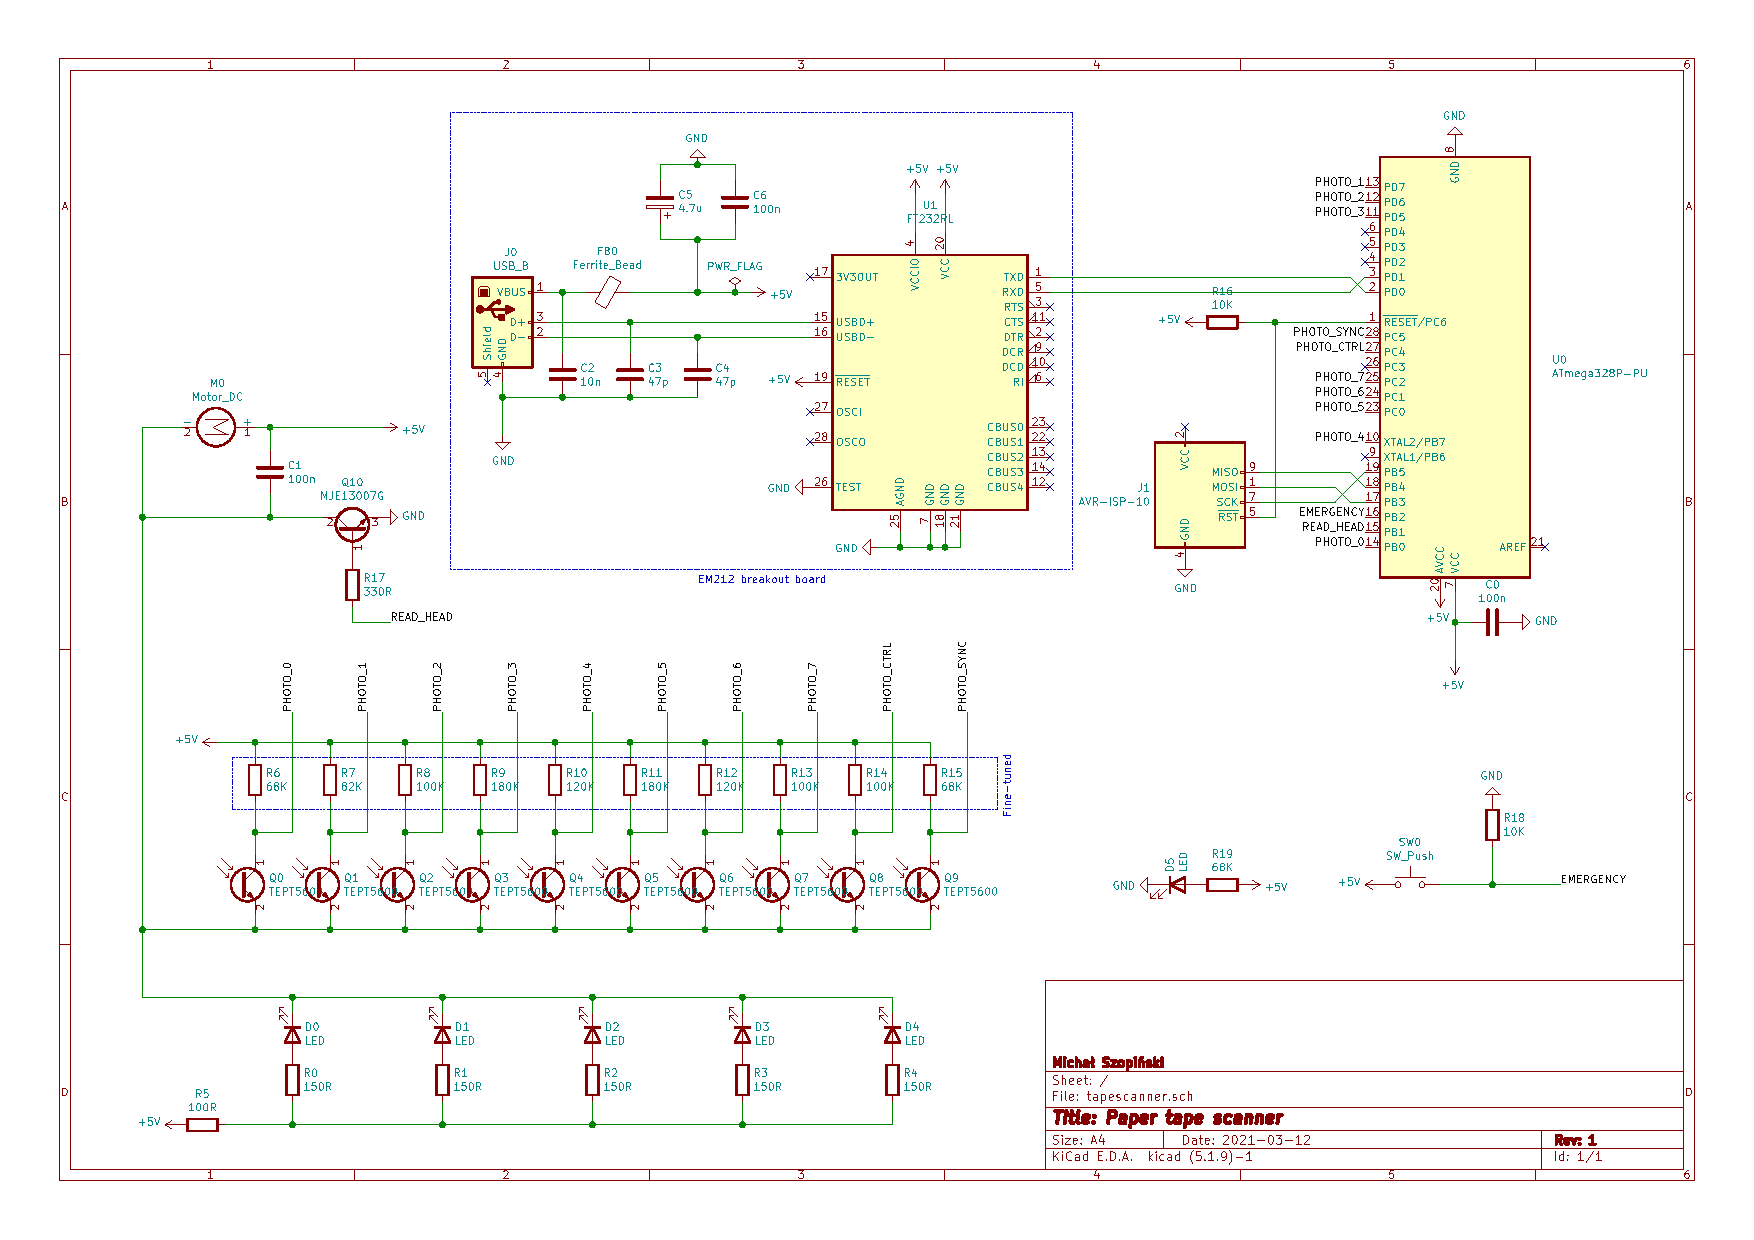
\includepdf[landscape]{img/schematic}
	
	\subsubsection{USB communication port and power source}
	
	Data transmission and power supply are done through the USB port placed on
	top of the FT232 breakout board designated as ``EM212". This board houses
	the chip itself as well as the noise filtering circuitry for both the power
	and the data lines.
	
	The power line is stabilized with a combination of a 4.7 \textmu F
	electrolytic capacitor and a 100 nF ceramic capacitor. This eliminates both
	low and high-frequency noise from the line. A ferrite bead connected in
	series with the line further reduces high-frequency noise.
	
	When operating as a USB to UART converter, the FT232 chip requires no
	additional circuitry and may be directly connected to the TXD and RXD pins
	of the microcontroller.
	
	\subsubsection{LED and phototransistor array}
	
	Due to insufficient voltage on the power rail, the light-emitting diodes
	must be connected in parallel rather than in series. To distribute the
	current evenly, each of the LEDs is given its own resistor. An additional
	100 \textOmega {} resistor connected in series with the power rail is used
	to adjust the brightness.
	
	The intensity of light reflected from the paper is probed using
	phototransistors. Each transistor-resistor pair can be thought of as a
	voltage divider of constant input and variable output. By default, in total
	darkness, no current flows through the transistor and the voltage is pulled
	high through the resistor. When the transistor is hit by light, current
	starts flowing from the collector to the emitter and from there to ground,
	reducing the voltage on the pin.
	
	Because of imperfections in the assembly process of the read head as well
	as varying sensitivity of the transistors, each of the resistors is
	fine-tuned to obtain a suitable intensity response characteristic. As a
	result, the array may be used to drive the pins of the microcontroller
	directly, without the need for amplification or analog-to-digital
	conversion.
	
	\subsubsection{Roller motor}
	
	As the sole mechanical component of the device, the DC motor is responsible
	for most of its power consumption. Consuming a current of up to 170 mA, the
	motor is nonetheless within the limits imposed by the USB standard, which
	mandates a maximum current of 500 mA. This does require the reader to be
	configured as a ``high-power" device, which is handled by the FT232 chip.
	
	To prevent noise to the power rail, a 100 nF capacitor is placed across the
	terminals of the motor. Power to the motor is controlled by a circuit
	described in the next subsection.
	
	\subsubsection{Power switching circuit}
	
	To decrease power consumption and reduce wear on the rubber roller, power
	to the read head is enabled on demand through an NPN power transistor.
	When enabled, the transistor shunts the ground rail of the head with the
	common ground.
	
	The base current is dictated by a 330 \textOmega {} resistor in series with
	the base. At 15 mA, the current may be sourced directly from the
	microcontroller without the need for a Darlington configuration.
	
	\subsubsection{User interface}
	
	Only two elements constitute the user interface: the power LED and the
	emergency stop button.
	
	The power LED is permanently connected between the power rail and the
	ground rail. Being a bright green LED, it only requires a 68 k\textOmega {}
	resistor to emit a substantial amount of light.
	
	The emergency stop button is a momentary push switch that shunts the
	emergency stop pin with the power rail. When the switch is not depressed,
	the pin is pulled low through a 10 k\textOmega {} resistor.
	
	\newpage
	\section{Firmware implementation}
	
	\subsection{Overview}
	\label{sec:firmoverview}
	
	To guarantee fluid operation and responsiveness of the physical and serial
	interfaces, the firmware is largely asynchronous in nature. This means that
	many operations are performed ``in the background" (through interrupts) and
	the main subroutine is often reduced to merely coordinating the exchange of
	data between interrupt handlers.
	
	That said, two major modes of operation may be discerned that were included
	in the main flow of execution. Those are \textit{standby mode} and
	\textit{session mode}. The device alternates between the two modes in
	response to various signals, including messages, user interaction and
	sensor input.
	
	Due to this asynchronicity, it is difficult to describe the entire
	algorithm in a single flowchart. For that reason, the many independent
	subroutines are grouped together by the context in which they are
	presented. This, however, is not the only peculiarity of the system.
	
	The firmware employs a system-wide exception handling mechanism. Because
	exceptions are a high-level concept, this feature is emulated by a global
	error status register. ``Throwing an exception" is performed by writing a
	non-zero value to this register.
	
	Any routine which calls an error-generating subroutine must check the error
	register after it returns and abort execution if the error status is
	non-zero. Any routine which stalls execution until a condition is met must
	also simultaneously check the value of the error register.
	
	Because error-handling code largely disregards the ordinary flow of
	execution while still being explicitly incorporated into the algorithm, the
	symbols representing this code are printed in red for clarity.
	
	\subsection{Top-level loop and main subroutine}
	
	Before any meaningful activity may begin, the device must be properly
	configured. This includes configuring the read head pin as an output,
	adjusting the timer to fire once per millisecond, setting the UART
	transciever to 9600 baud and enabling global interrupts.
	
	\begin{figure}[h]
		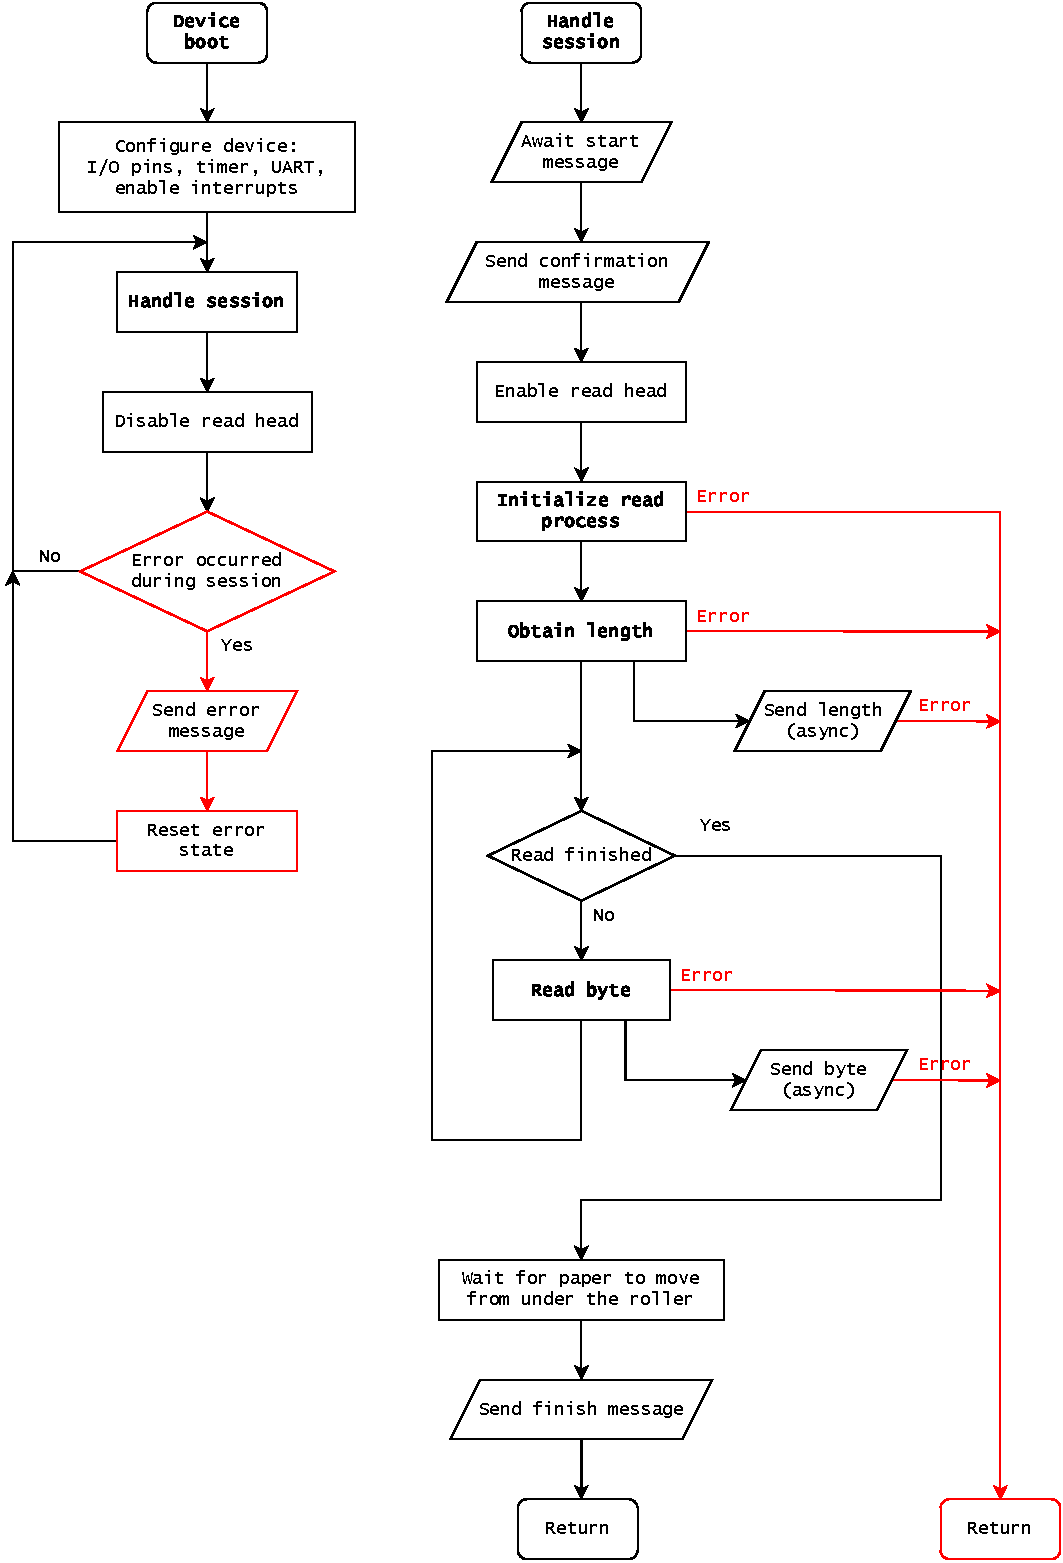
\includegraphics[width=\linewidth]{img/main}
		\caption{The top-level loop and the main subroutine.}
	\end{figure}
	\clearpage
	
	Following the configuration, the top-level loop begins. The inside of the
	loop houses the global error handler and may be interpreted as a
	``try-catch-finally" statement known from higher-level languages. First,
	the main subroutine is called to perform its duties. Regardless of the
	outcome, power to the read head is disabled once it returns. If an error
	caused the main routine to abort, an error message is sent, the error
	register is cleared and the loop reiterates.
	
	The main subroutine contains the entire algorithm for reading data tapes.
	It begins by polling the serial interface for a start message (see
	table~\ref{sec:messages}). Once received, the device responds with a
	confirmation message and enables power to the read head. It is at this
	point that the transition from standby mode to session mode occurs.
	
	With the LEDs powered on and the roller motor running, the initialization
	process begins. The device waits a certain amount of time for the first
	symbol to appear. If the initialization times out, the session is aborted.
	
	Once the first symbol has appeared, the length header (described in
	section~\ref{sec:format}) is scanned. Upon completion, the newly discovered
	length is queued for asynchronous transmission, which is depicted in the
	diagram as a branch separating from the main flow. Following this, the
	remaining bytes are also read and asynchronously transmitted.
	
	Finally, after all the bytes have been read, the device retains power to
	the read head for a short amount of time to remove the paper tape from
	under the roller. Once the timeout clears, a ``read finished" message is
	sent and the device reenters standby mode.
	
	\subsection{Binary data recovery algorithm}
	\label{sec:readalg}
	
	In order to design an effective algorithm which recovers binary data from
	the analog input signal, it is important to understand how changes in light
	intensity affect the voltage levels visible to the device. Below is a
	oscillogram depicting the readout of a sample data track.
	
	\clearpage
	
	\begin{figure}[h]
		\begin{center}
			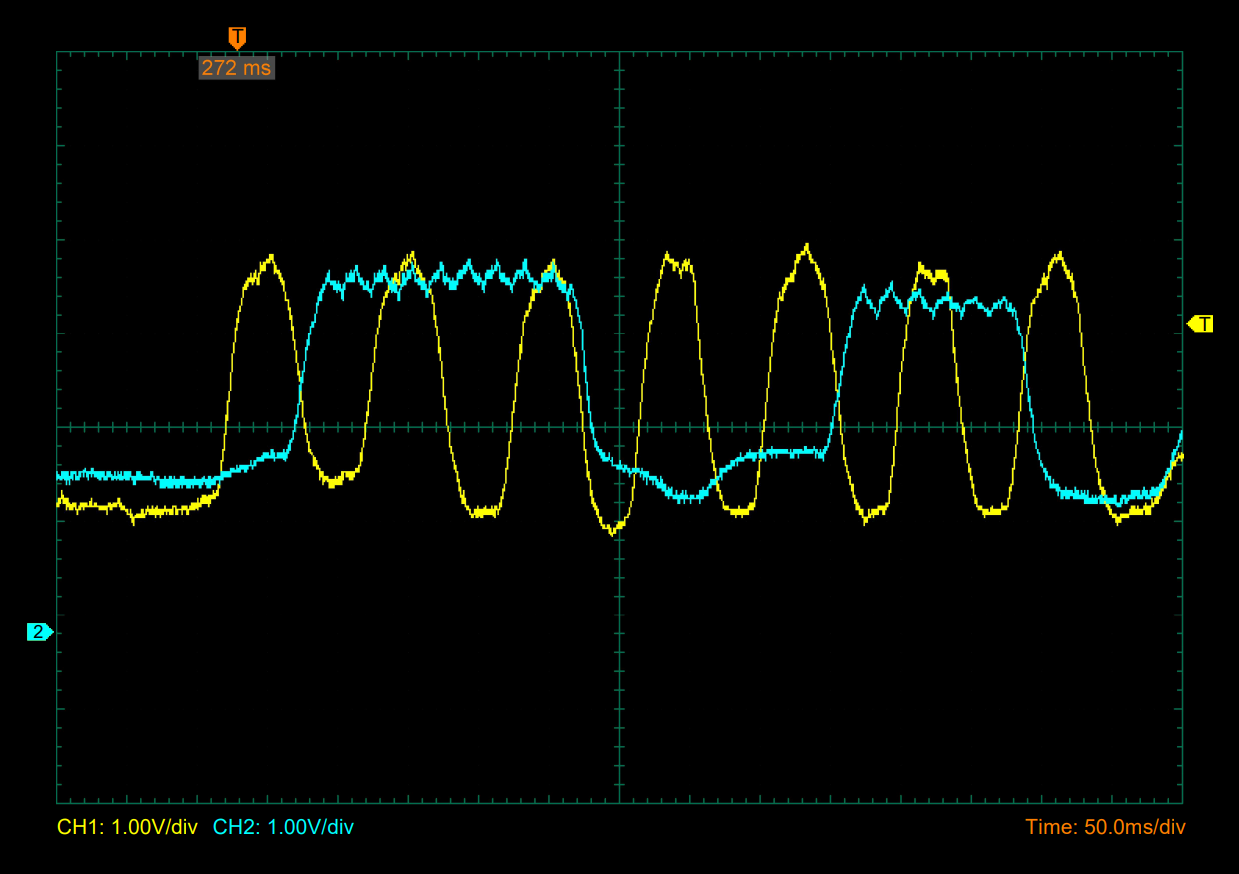
\includegraphics[width=0.6\linewidth]{img/osc1}
			\caption{Voltage levels generated by the signal
			\texttt{0111100001110}. Yellow signal: sync track, blue signal:
			data track.}
		\end{center}
	\end{figure}
	
	\begin{figure}[h]
		\begin{center}
			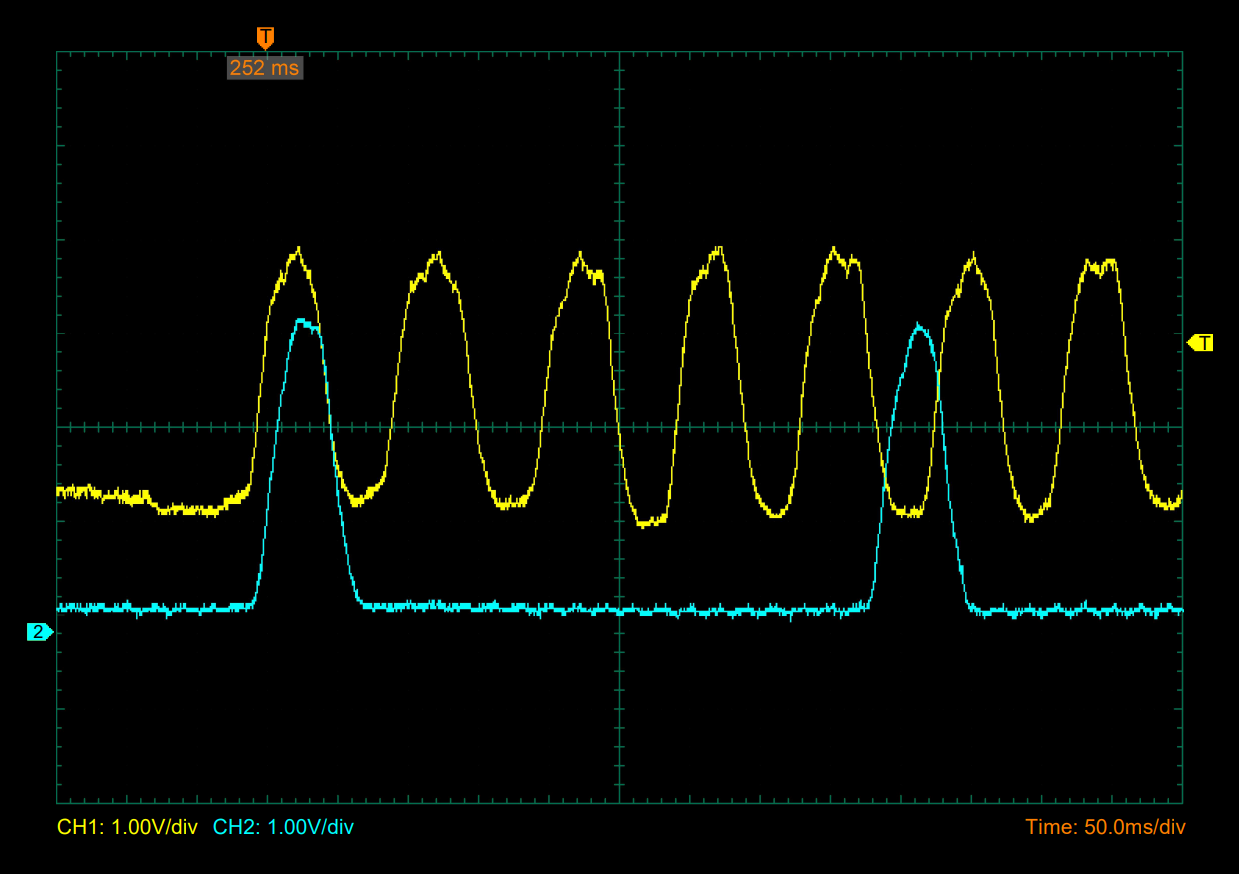
\includegraphics[width=0.6\linewidth]{img/osc2}
			\caption{Different signal unaffected by neighboring tracks,
			exhibiting a phase shift.}
		\end{center}
	\end{figure}
	
	As may be noted, voltage levels change rapidly near the edges of the sync
	signal and stabilize towards the end of its ridges and valleys.
	Furthermore, they are affected by neighboring data tracks and they exhibit
	a slight phase shift relative to the sync signal. As such, there is only a
	short time window in which all 10 of the data tracks may be accurately
	read.
	
	A heuristic approach that proved effective in data recovery was to probe
	the symbol at about 68\% ($\frac{11}{16}$) of its duration. This involves
	sampling the signal evenly over an extended period of time and only picking
	a sample once the symbol has ended and its duration is known. This
	algorithm was chosen to be implemented in the firmware.
	
	\subsection{Implementation details}
	
	\subsubsection{Two-step initialization}
	\label{sec:init}
	
	\begin{figure}[h]
		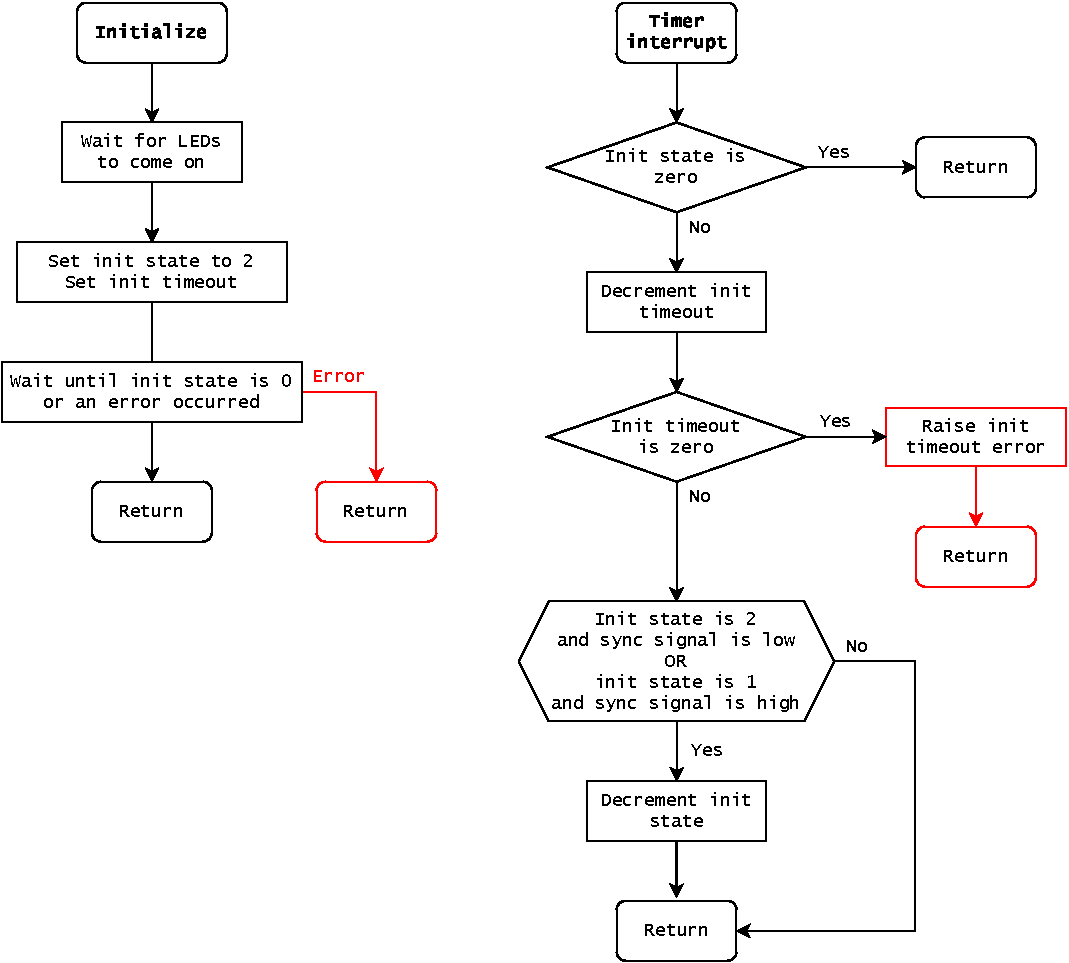
\includegraphics[width=\linewidth]{img/init}
		\caption{The initialization subroutine and interrupt handler.}
	\end{figure}
	
	The two-step initialization subroutine called at the start of the read
	session waits until the first symbol appears. This is done by inspecting
	the sync signal and awaiting a high logic state. To handle unpredictable
	logic levels before the tape is inserted into the reader, a low sync signal
	must be detected first.
	
	The routine implements the ``coordinator" pattern commonly observed
	throughout the system whereas the main logic is delegated to an interrupt
	handler while the parent function stalls execution until a condition is
	met.
	
	\newpage
	\subsubsection{Read byte subroutine}
	
	\begin{figure}[h]
		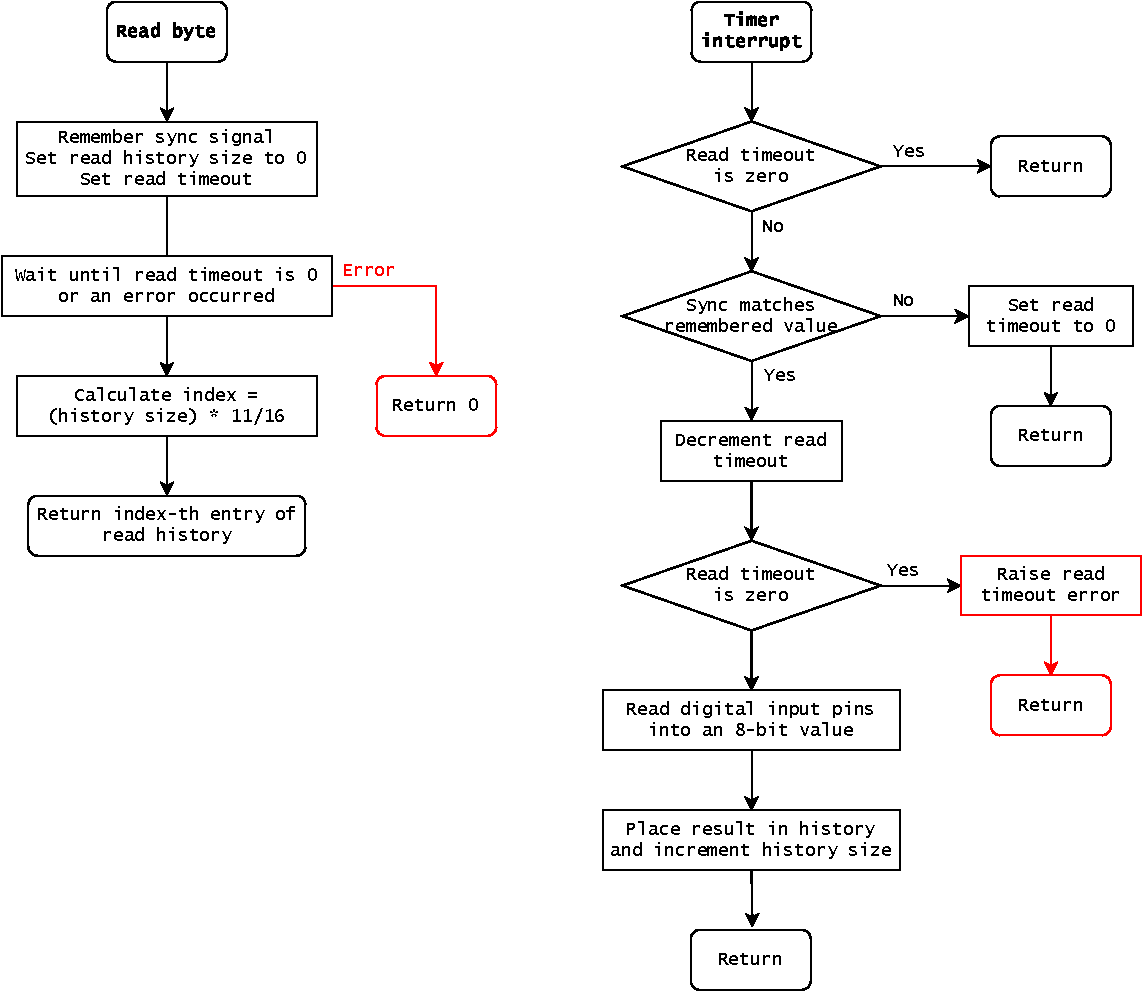
\includegraphics[width=\linewidth]{img/read}
		\caption{The read subroutine and interrupt handler.}
	\end{figure}
	
	This is an implementation of the algorithm described in
	section~\ref{sec:readalg}. Thanks to the initialization subroutine, the
	algorithm is guaranteed to start at the very beginning of the first symbol.
	The subroutine returns once the end of the symbol is reached, after which
	it is immediately called again.
	
	\newpage
	\subsubsection{Synchronous IO}
	
	\begin{figure}[h]
		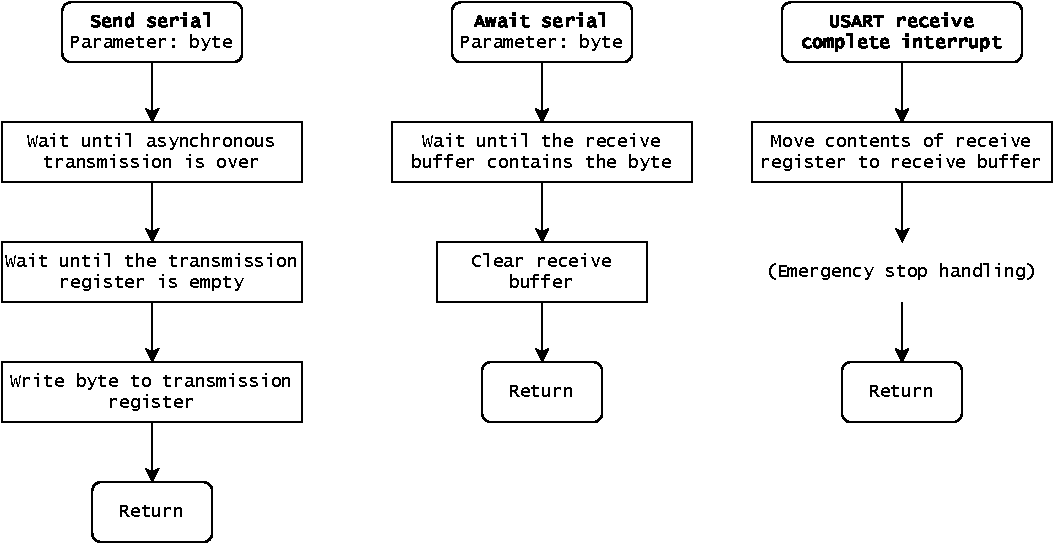
\includegraphics[width=\linewidth]{img/sync}
		\caption{The synchronous I/O procedures and interrupt handler.}
	\end{figure}
	
	The synchronous send procedure stalls execution until it's clear to send
	the specified byte. The await procedure stalls execution until the
	specified byte is received. No error handling is implemented because the
	procedures are only used at the very start and end of a session, where the
	opportunities for an error are scarce.
	
	Note that the await procedure uses a receive buffer which is separate from
	the hardware UART receive register. This behavior is unrelated to the I/O
	procedures themselves, but it is needed for emergency stop handling (see
	section~\ref{sec:estop}).
	
	\newpage
	\subsubsection{Asynchronous IO}
	
	\begin{figure}[h]
		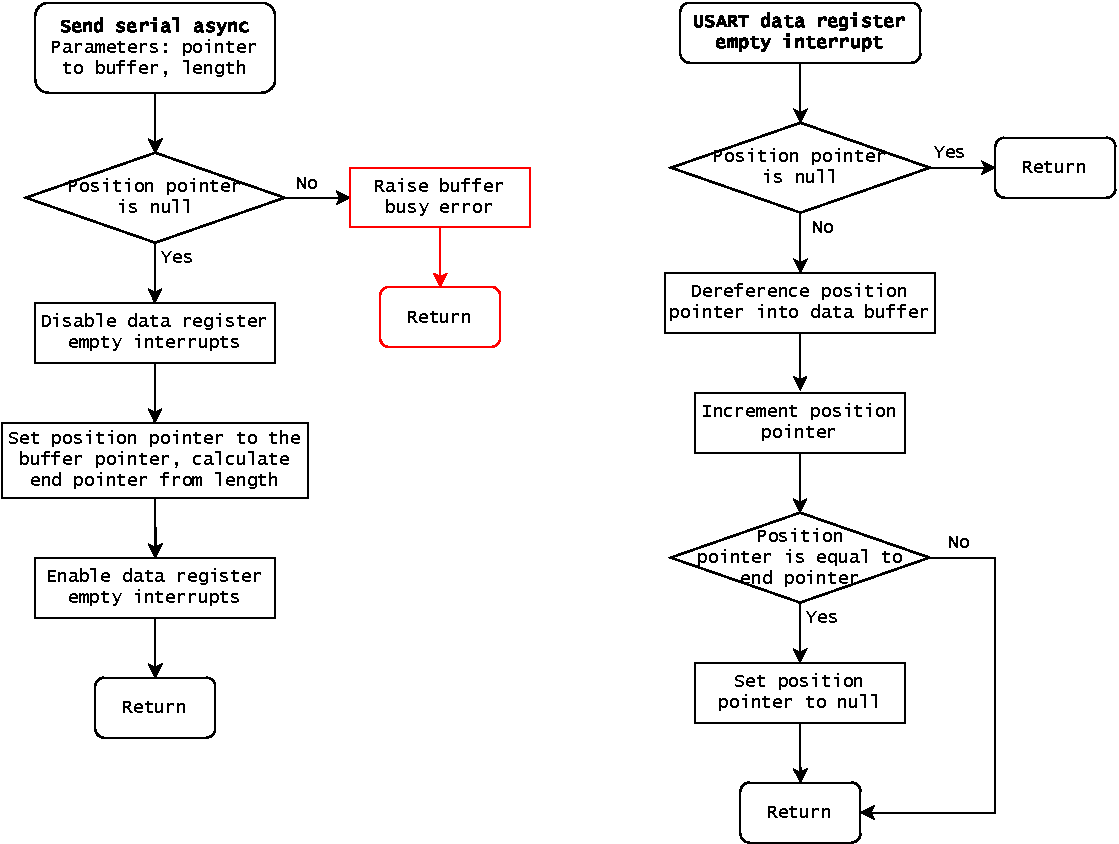
\includegraphics[width=\linewidth]{img/async}
		\caption{The asynchronous I/O procedure and interrupt handler.}
	\end{figure}
	
	The asynchronous send procedure is designed to send large amounts of data
	without stalling the execution of the main routine. It iterates over an
	externally allocated buffer and transmits the specified number of bytes.
	
	An error is raised when an attempt to start transmission is made before the
	previous transmission completes. To prevent race conditions, register empty
	interrupts are temporarily disabled while the transmission parameters are
	being set. Reenabling the interrupts immediately triggers the handler.
	
	\newpage
	\subsubsection{Emergency stop}
	\label{sec:estop}
	
	\begin{figure}[h]
		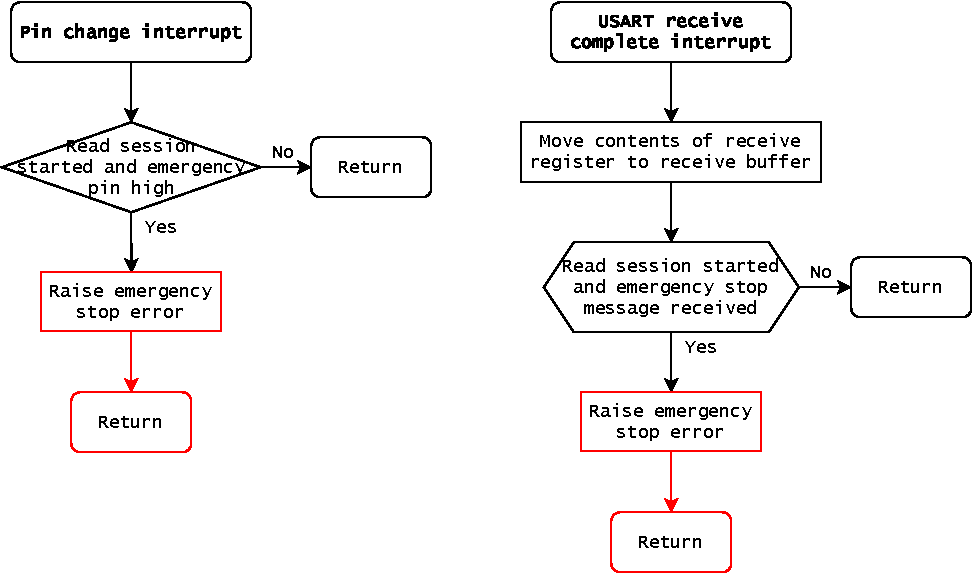
\includegraphics[width=\linewidth]{img/estop}
		\caption{The emergency stop interrupt handlers.}
	\end{figure}
	
	The emergency stop interrupt handlers listen to both possible sources of
	stop signals and raise the emergency stop error, aborting the main routine
	through mechanisms described in section~\ref{sec:firmoverview}. The USART
	handler intercepts all traffic before it is handled by the I/O subroutines.
	Because reading from the USART data register clears it, its contents must
	be moved to a separate buffer before the handler returns.
	
\end{document}
